Brains do remarkable work in actively analyzing environmental information and making decisions based on this information. Among all brain systems, sensory systems are especially concentrated on analyzing some particular environmental information, e.g., light for visual systems, sound for auditory systems, and inputs from whiskers for the rodent somatosensory systems~\cite{purves2001neuroscience}.
The goal of these sensory systems is to extract behaviorally useful information from the complex raw input data, a process which could be described as untangling the behavior-related dimensions (such as category) from other orthogonal dimensions (such as translation and rotation of the objects)~\cite{yamins2016using}.
While these systems radically differ in their input modalities, number of overall neurons, and specific neuronal microcircuits, most of them share two fundamental characteristics. First, they are deep sensory cascades, consisting of sequences of brain areas (cortical and subcortical), each of which alone is comparatively simple, but which together produce a complex transformation of the input data. Second most of them are inherently spatially extended~\cite{felleman1991distributed}.
In this paper, we will propose a method to give a computational model for the rodent somatosensory systems based on the hierarchical structure and the function of untangling.

Similar to the ventral stream of visual systems with hierarchical structures from V1, to V2, V4, and IT~\cite{felleman1991distributed, Goodale1992}, researchers have found evidence showing hierarchical processing for somatosensory input in rodents, human, and primates\cite{Pons1987, Inui2004, Iwamura1998}. For example, the second somatosensory area (S2) is found to rely on inputs from S1 (first somatosensory area) \cite{Pons1987, Petersen2007}. And barrel cortex, S1, and S2 are also found to get different aspects of input from rodent whiskers \cite{Diamond2008}. Meanwhile connections between barrel cortex and S1, S1 and S2 are also believed to convey information for hierarchical processing \cite{Petersen2007}. However, while barrel cortex is already explored a lot, the functions of both S1 and S2 is poorly understood.

In this work, we will use hierarchical models for rodent somatosensory systems as a computational model that correctly describes neural responses as a function of stimulus input.
Hierarchical models are also used widely in artificial intelligence to help design better systems for various tasks. Recent work using deep neural networks (DNNs) has achieved significant improvements on object recognition, speech recognition, and numerous other artificial intelligence tasks\cite{Krizhevsky, hinton2012deep, lecun2015deep}.
These deep neural networks are all composed of multiple simple neural network layers in series, where the computation in single layer is usually simple but non-linear and stacks of those simple non-linear computations make up a highly complicated non-linear computation.
DNNs are also believed to be biologically plausible, and therefore could be good candidates for models of sensory cortical brain systems.

In fact, researchers have also found that the DNNs optimized for performances on object recognition tasks serve as a good model for the primate ventral visual stream \cite{Yamins2013, Yamins2014, cadieu2014deep}.
Using a general class of computational architectures known as HCNNs \cite{lecun1995convolutional}, which also include the recent convolutional neural networks, they found that optimizing for object recognition task could improve not only the performances on explaining the responses of IT layers using that of final layers but also that of explaining V4 areas using intermediate layers of the same architecture simultaneously \cite{cadieu2014deep}.
And the final models they got successfully surpassed all existed models on explaining IT and V4 areas. Similar results were also found in the deep neural networks that were trained on large-scale object recognition tasks \cite{Yamins2014}.

\begin{figure}
\centering
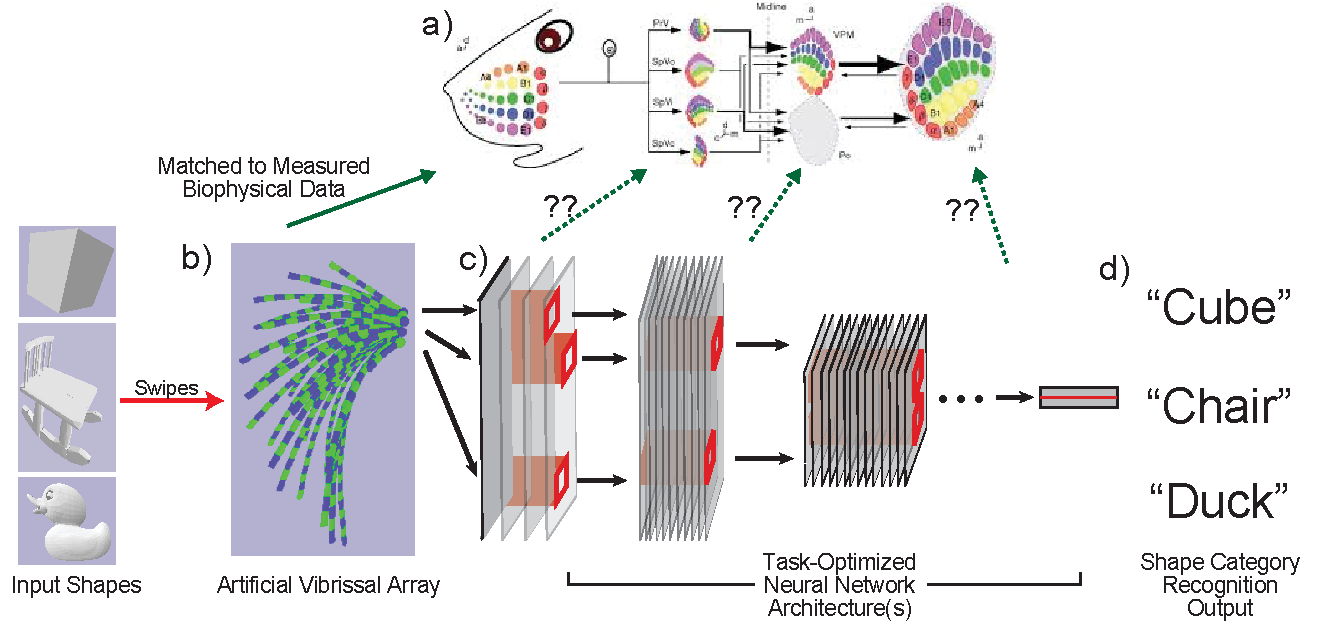
\includegraphics [width=1\linewidth]{figures/schematic.pdf}
\vspace{-2mm}
\caption{\textbf{Goal-Driven Approach to Modeling Barrel Cortex:} \textbf{a.} Rodents have highly sensitive whisker arrays that provide input data about the animal's environment.  Whisker signals are is subsequently processed by a somatosensory cascade of brain areas knowns as barrel cortex. Barrel cortex is a prime target for modeling because it is likely to be richly representational, but its computational underpinnings are largely unknown. Our long-term approach to modeling barrel cortex is \emph{goal-driven}: using an artificial whisker-array input device built using extensive biophysical measurements (\textbf{b.}), we seek to optimize neural networks of various architectures (\textbf{c.}) to solve ethologically-relevant shape recognition tasks (\textbf{d.}), and then measure to what extent the networks predict fine-grained response patterns in real neural recordings. ~\label{fig_schematic}}
\end{figure}



Utilizing the goal-driven modeling method which has been proven to be successful for visual ventral stream, we will show how we can use hierarchical models for modeling the rodent somatosensory systems.
In order to do that, we need to first have a large-scale dataset for training the DNNs.
The dataset is supposed to teach the DNNs to perform the tasks that rodent somatosensory systems are doing using the responses from whisker arrays.
Therefore, the dataset should simulate the situations faced by rodent somatosensory systems as similar as possible. 
Nevertheless, it is impossible to directly collect the data from real whisker arrays as the data required is too much, so we decide to build a virtual whisker array which is supposed to be as similar as real arrays both in static shapes and dynamic behaviors during the collision with other objects.
Given that, we then need to find the tasks performed by rodent somatosensory systems to help design the dataset. 
For example, if we believe the task is object recognition, then we should use whisker array to sense different objects and the DNNs should be trained to predict the labels from the responses.
However, what rodent somatosensory systems are doing is still unknown, while there are many possible candidates, including detecting object shape, position, and texture of object surface\cite{Boubenec2012,Diamond2008,Arabzadeh2005,OConnor2010}.
In this paper, we will work with the assumption of object recognition, while the dataset will also be available for other tasks. 
Based on that, we generate a large-scale dataset and then train DNNs with different structures corresponding to different hypotheses of the computations done by neurons in the somatosensory cortex.
After the DNNs trained, one will need a neural response dataset which is collected from neurons in rodent somatosensory systems to examine the performances of neural fitting by these networks as well as distinguish different network structures.
Nonetheless, this kind of dataset has not been availabel. Hence we use the performances on the dataset with current task to try to do the comparisions between various structures under the assumption that the better the network is on the task, the better it will be to predict neural responses, as did for models of visual ventral stream.

In summary, we will show how to use goal-driven modeling method for rodent somatosensory systems. In next few sections, we will show how we build the virtual whisker array, generate the dataset, and train the networks. Our codes for the whisker array and dataset will also be availabel in public later.

